\documentclass[aspectratio=169,dvipsnames]{beamer}
\usepackage[utf8]{inputenc}
\usepackage[english]{babel}
\usepackage{graphicx,hyperref,icmc,url}
\usepackage{subcaption}
\usepackage{multirow}
\usepackage{minted}
\usepackage{listings}
\usepackage{tikz}
\usepackage{array}
\usepackage{xcolor, soul}
\usepackage{mathtools}

\usepackage{fontawesome5}




\usepackage{listings}% http://ctan.org/pkg/listings
\usepackage{graphbox}
\usepackage{booktabs}
\usetikzlibrary{positioning}

\newcommand{\destaq}[1]{\textcolor{BlueViolet}{\textbf{#1}}}
\newcommand\todo[1]{\colorbox{green}{#1}}

\definecolor{echodrk}{HTML}{0099cc}
\definecolor{olivegreen}{rgb}{0,0.6,0}
\definecolor{camdrk}{RGB}{0,62,114}

\usetikzlibrary{arrows,shapes,arrows.meta}

\definecolor{mygreen}{rgb}{0,0.6,0}

\definecolor{mymauve}{rgb}{0.58,0,0.82}

\usetikzlibrary{arrows,shapes, decorations.pathmorphing,backgrounds,positioning}

\pgfdeclarelayer{background}
\pgfsetlayers{background,main}

\tikzstyle{vertex}=[circle,fill=black!25,minimum size=20pt,inner sep=0pt]
\tikzstyle{selected vertex} = [vertex, fill=red!24]
\tikzstyle{select vertex} = [vertex, fill=blue!24]
\tikzstyle{selectx vertex} = [vertex, fill=green!24]
\tikzstyle{edge} = [draw,thick,-]
\tikzstyle{selected edge} = [draw,line width=5pt,-,red!50]


% The title of the presentation:
%  - first a short version which is visible at the bottom of each slide;
%  - second the full title shown on the title slide;
\title[Spectral GNNs vs GAT
]{Spectral GNNs vs GATs \\ When attention is (not all you need) the "only" option
}

% Optional: a subtitle to be displayed on the title slide


% The author(s) of the presentation:
%  - again first a short version to be displayed at the bottom;
%  - next the full list of authors, which may include contact information;
\author[Jorge Luiz Franco]{Jorge Luiz Franco\\ \bigskip
\textsc{Complex Networks for Computer Science}\\ \bigskip
Professor: Diego Amancio, Ph.D.}

% \\ \bigskip
    % \large{}

% The institute:
%  - to start the name of the university as displayed on the top of each slide
%    this can be adjusted such that you can also create a Dutch version
%  - next the institute information as displayed on the title slide
\institute[ICMC/USP]{Universidade de São Paulo - ICMC}

% Add a date and possibly the name of the event to the slides
%  - again first a short version to be shown at the bottom of each slide
%  - second the full date and event name for the title slide
\date[2024]{\footnotesize{Nov 3, 2024}}

\sloppy

\AtBeginSection[]
{
    \begin{frame}<beamer>{Summary}
        \tableofcontents[currentsection]
    \end{frame}
}

\begin{document}

    \begin{frame}[plain]
        \titlepage
    \end{frame}

    \begin{frame}
      \frametitle{Summary}
      \tableofcontents
    \end{frame}

%%%%%%%%%%%%%%%%%%%%%%%%%%%%%%%%%%%%%%%%%%%%%%%%%%%%%%%%%%%%%%%%

% Introduction
% Materials and Methods
%   Datasets
%   MST
%   OPF
% Experiments
%   Initial
%   DTW
%   Pruning and Improvements
%   Batch-Tests
%   Results
%   Difficulties, limitations, and future works

\section{Introduction}

\begin{frame}{Motivation}
\begin{itemize}
    \item Growing importance of efficient last-mile delivery logistics.
    \item Use of drones (Unmanned Aerial Vehicles, UAVs) for overcoming traffic constraints, reducing delivery times, and lowering operational costs.
    \item Significant increase in literature on Delivery Drones in recent years \cite{DUKKANCI2023}.
\end{itemize}
\end{frame}

\begin{frame}{Introduction to Last-Mile Delivery Drones}
    \begin{figure}
      \begin{columns}
        \column{.3\linewidth}
        \caption{Drones Congestion in a high-traffic Last Mile Delivery context. \\ Source: \cite{imageDronesCongestion}}
        \label{fig:example left}
        \column{.65\linewidth}
        \includegraphics[width=\textwidth]{img/Drone Congestion.jpg}
      \end{columns}
    \end{figure}

\end{frame}

\begin{frame}{Introduction to Last-Mile Delivery Drones}
\destaq{Last Mile Delivery Drones (LMDD)}
\begin{itemize}
    \item Heterogeneous research area:
    \begin{itemize}
        \item Combining drones and trucks.
        \item Linear integer modeling.
        \item Fuzzy logic for uncertainties.
        \item Multi-objective optimization.
        \item Exclusive drone-based solutions.
    \end{itemize}
    \item \textbf{Complex Systems Decentralized Approach}:
    \begin{itemize}
        \item Tradable permit model for multi-agent airspace use \cite{Verri}.
    \end{itemize}
\end{itemize}

\end{frame}

\begin{frame}{Related Work and Centralized Control}
\begin{itemize}
    \item \textbf{Necessity of Air Traffic Management}:
    \begin{itemize}
        \item Most centralized models don't address collision avoidance \cite{DUKKANCI2023}.
        \item Ensuring optimal path planning and efficient airspace control.
    \end{itemize}
    \item \textbf{Centralized Control and UTM}:
    \begin{itemize}
        \item \textbf{Centralized Control}:
        \begin{itemize}
            \item Federal Aviation Administration (FAA) and NASA's Unmanned Aircraft System Traffic Management (UTM) \cite{nasa}.
            \item Ensures organized, legislative-backed airspace control.
        \end{itemize}
        \item \textbf{Decentralized Models}:
        \begin{itemize}
            \item Novel but complex in scalability and regulatory compliance.
        \end{itemize}
    \end{itemize}
\end{itemize}
\end{frame}


\begin{frame}{Proposed Approach}
\begin{itemize}
    \item \textbf{Aispace Control and MAPF Approach}:
    \begin{itemize}
        \item Multi-Agent Path Finding (MAPF) is a solution for addressing spatial characteristics and collision avoidance.
    \end{itemize}
    \item \textbf{Proposed Strategy}:
    \begin{itemize}
        \item Employing MAPF strategy for Last Mile Delivery Drone problem.
        \item Three approaches: MILP, heuristic and hybrid.
        \item Use of prioritized planning \cite{7138650} and conflict-based search \cite{SHARON201540} to manage computational complexity in the heuristic.
        \item Comparing the MILP with the heuristic.
        \item Qualitative comparison between centralized and decentralized approaches.
    \end{itemize}
\end{itemize}
\end{frame}




\section{Spectral GNNs}

\begin{frame}{Spectral GNNs}
    \destaq{Introduction to Spectral GNNs}
    \begin{itemize}
        \item Spectral Graph Neural Networks derived from GSP principles.
        \item \textbf{Key Concept}: Graph Laplacian $\mathcal{L} = D - A$ (degree matrix $D$ and adjacency matrix $A$) captures graph structure, enabling spectral operations analogous to Fourier transforms.
        \item Objective: Represent node features as signals on a graph.
        \item Spectral Methods:
        \begin{itemize}
            \item \textbf{Eigenvalue-based}: Filters created in Fourier domain.
            \item \textbf{Eigenvector-based}: Decomposition of signals via spectral basis \cite{bo2023surveyspectralgraphneural}.
        \end{itemize}
    \end{itemize}
\end{frame}

\begin{frame}{Spectral CNN (SCNN)}
    \destaq{First Spectral GNN - Spectral CNN (SCNN)}
    \begin{itemize}
        \item \textbf{Concept}: Transforms CNN concepts from images to graphs.
        \item \textbf{Mathematics}:
        \begin{itemize}
            \item Graph Fourier Transform: $\hat{f} = U^T f$
            \item Convolution: $g_{\theta} \star f = U g_{\theta} U^T f$, where $U$ and $\Lambda$ are derived from $\mathcal{L} = U \Lambda U^T$.
            \item \textbf{Challenges}:
            \begin{itemize}
                \item High computational cost $\mathcal{O}(n^3)$.
                \item Non-localized eigenvectors can overshadow local details \cite{bruna2013spectral}.
            \end{itemize}
        \end{itemize}
    \end{itemize}
\end{frame}

\begin{frame}{Graph Laplacian Spectra}
    \begin{figure}
      \begin{columns}
        \column{.3\linewidth}
        \caption{Eigenvectors as signals denotes nodal regions of eigenvalues of the graph Laplacian.}
        \label{fig:graph_spectra}
        \column{.65\linewidth}
        \includegraphics[width=\textwidth]{img/graph_spectra.png}
      \end{columns}
    \end{figure}

\end{frame}


\begin{frame}{ChebNet}
    \destaq{ChebNet - Addressing SCNN Limitations}
    \begin{itemize}
        \item \textbf{Introduction of Chebyshev Polynomials}:
        \begin{itemize}
            \item Approximates spectral filters for reduced computational demands using Chebyshev polynomials.
            \item Defines filters as: $ g_{\theta}(\mathcal{L} ) f = \sum_{k=0}^{K-1} \theta_k T_k(\widetilde{\mathcal{L}}) f $.
            \item Scaled Laplacian: $\widetilde{\mathcal{L}} = 2 \frac{\mathcal{L}}{\lambda_\text{max}} - I_n$.
        \end{itemize}
        \item \textbf{Advantages}:
        \begin{itemize}
            \item \textbf{Scalability}: Only first eigenpair needed ($\mathcal{O}(n^2)$ via power method).
            \item \textbf{Localized Filtering}: $K$-localized for $K^{th}$-order polynomial filters, representing paths up to length $K$ \cite{defferrard2016convolutional}.
        \end{itemize}
    \end{itemize}
\end{frame}

\begin{frame}{Graph Convolutional Networks (GCNs)}
    \destaq{Graph Convolutional Networks (GCNs) - A Simplified Approach}
    \begin{itemize}
        \item \textbf{GCN Concept}:
        \begin{itemize}
            \item Rooted in Chebyshev expansion truncation ($K=1$), focusing on first-order neighbors.
            \item Propagation Rule: $g_{\theta} \star f \approx \theta (I_n + \widetilde{A}) f$ with $\widetilde{A} = D^{-\frac{1}{2}} A D^{-\frac{1}{2}}$.
        \end{itemize}
        \item \textbf{Benefits}:
        \begin{itemize}
            \item Simplifies computation while remaining effective.
            \item Often categorized as a spatial method due to neighborhood aggregation \cite{kipf2016semi}, \cite{wu2019simplifying}.
        \end{itemize}
    \end{itemize}
\end{frame}

\begin{frame}{GCN diagram}
    \begin{figure}[h]
    \centering
    \begin{columns}

    \column{.25\linewidth}

    \caption{Graph Convolution updating node embedding $\vec{h_b}$}

    \label{fig:visualgo}

    \column{.75\linewidth}
    \resizebox{0.975\columnwidth}{0.455\linewidth}{%

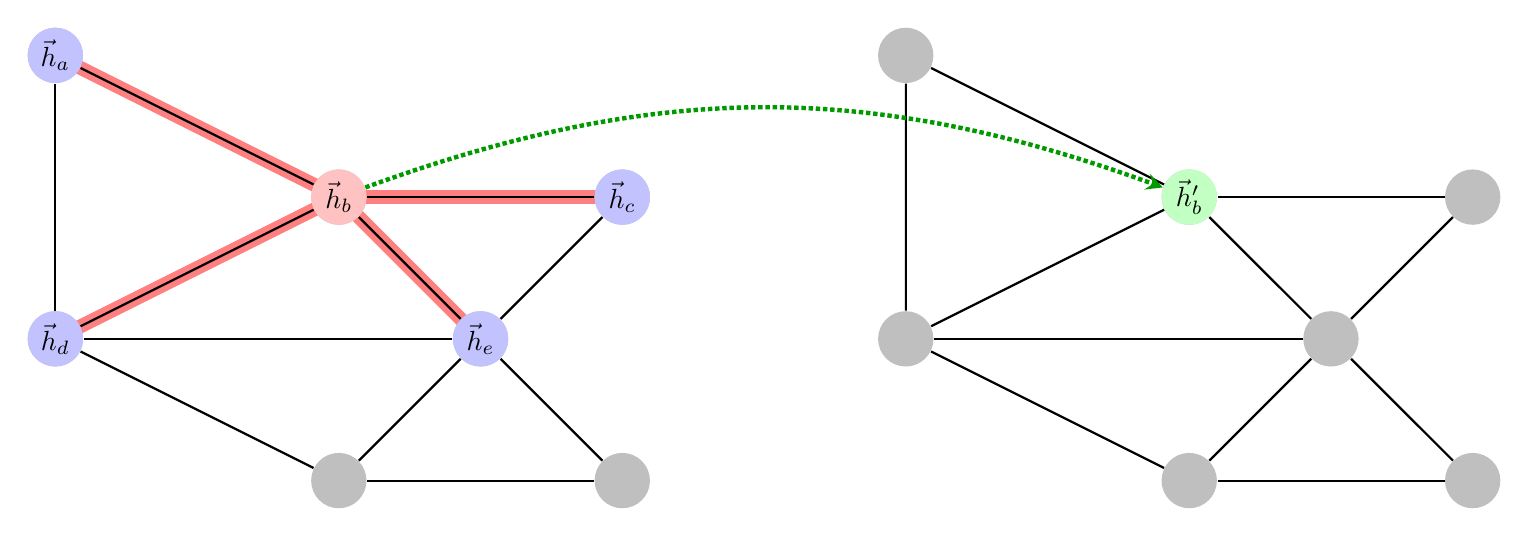
\begin{tikzpicture}[scale=1.8, auto,swap]
    \foreach \pos/\name in {{(0,2)/a}, {(2,1)/b}, {(4,1)/c},
                            {(0,0)/d}, {(3,0)/e}, {(2,-1)/f}, {(4,-1)/g}}
        \node[vertex] (\name) at \pos {};

    \foreach \source/ \dest /\weight in {b/a/7, c/b/8,d/a/5,d/b/9,
                                         e/b/7, e/c/5,e/d/15,
                                         f/d/6,f/e/8,
                                         g/e/9,g/f/11}
        \path[edge] (\source) -- (\dest);

    \foreach \vertex / \fr in {b/4}
        \path node[selected vertex] at (\vertex) {$\vec{h}_b$};
    \foreach \vertex / \fr in {a/4, c/4, d/4, e/5}
        \path node[select vertex] at (\vertex) {$\vec{h}_{\vertex}$};
    \begin{pgfonlayer}{background}
        \foreach \source / \dest in {b/c,d/b,a/b,b/e}
            \path[selected edge] (\source.center) -- (\dest.center);
    \end{pgfonlayer}

    \foreach \pos/\name in {{(6,2)/a1}, {(8,1)/b1}, {(10,1)/c1},
                            {(6,0)/d1}, {(9,0)/e1}, {(8,-1)/f1}, {(10,-1)/g1}}
        \node[vertex] (\name) at \pos {};
    \foreach \source/ \dest /\weight in {b1/a1/7, c1/b1/8,d1/a1/5,d1/b1/9,
                                         e1/b1/7, e1/c1/5,e1/d1/15,
                                         f1/d1/6,f1/e1/8,
                                         g1/e1/9,g1/f1/11}
        \path[edge] (\source) -- (\dest);
    \foreach \vertex / \fr in {b1/4}
        \path node[selectx vertex] at (\vertex) {$\vec{h}'_b$};

    \draw[-stealth, densely dotted, ultra thick, mygreen] (b) edge[bend left=20] (b1);
\end{tikzpicture}


}
\end{columns}
\end{figure}

\end{frame}

\begin{frame}{Limitations of Spectral Methods}
    \destaq{Limitations of Spectral Methods}
    \begin{itemize}
        \item Restriction: Spectral GNNs typically work only on undirected graphs as they rely on symmetric spectral decomposition.

        \item Scalability: GCNs apart, spectral methods tend to be computationally expensive for large graphs.

        \item The nature of the adjacency matrix enforces `node-centric' approaches that may not be suitable for all tasks.

    \end{itemize}
\end{frame}

\section{Spatial GNNs}


\begin{frame}{Spatial-based GNNs Overview}
    \begin{itemize}
        \item Spatial-based GNNs perform convolutions in the spatial domain by directly leveraging the graph structure.
        \item These methods aggregate features from local neighborhoods, similar to CNNs on image data.
        \item Each node's features are updated iteratively through message passing with its neighboring nodes.
        \item Suitable for large-scale graphs due to their scalability and flexibility.
    \end{itemize}
\end{frame}

\begin{frame}{Message Passing Framework for Spatial GNNs}
    \begin{itemize}
        \item At layer \( t \), each node \( i \) aggregates features from its neighbors \( \mathcal{N}(i) \).
        \[
        \mathbf{m}_i^{(t+1)} = \text{AGGREGATE}^{(t)} \left( \left\{ \mathbf{h}_j^{(t)} : j \in \mathcal{N}(i) \right\} \right)
        \]
        \item Node \( i \) then updates its own features based on the aggregated message:
        \[
        \mathbf{h}_i^{(t+1)} = \text{UPDATE}^{(t)} \left( \mathbf{h}_i^{(t)}, \mathbf{m}_i^{(t+1)} \right)
        \]
        \item Flexible, adaptable to dynamic graphs, as they only require local neighborhood information.
    \end{itemize}
\end{frame}

\begin{frame}{Message Passing Diagram}

    \input{img/mpnn.tex}

\end{frame}


\begin{frame}{GraphSAGE: Sampling and Aggregation}
    \begin{itemize}
        \item GraphSAGE \cite{hamilton2017inductive} computes node embeddings by sampling and aggregating neighbor features.
        \item Various aggregation functions (e.g., mean, LSTM-based, pooling) allow flexibility for large graphs.
        \item Supports inductive learning by enabling embeddings for unseen nodes.
        \item Advantages:
            \begin{itemize}
                \item Inductive capability for new nodes.
                \item More scalable than spectral-based GNNs for large graphs.
            \end{itemize}
    \end{itemize}
\end{frame}

\begin{frame}{Graph Attention Networks (GAT)}
    \begin{itemize}
        \item GAT \cite{velickovic2017graph} introduces attention mechanisms to learn different weights for neighbors.
        \item Attention coefficient between nodes \( i \) and \( j \):
        \[
        c_{ij} = \phi_1 \left( \mathbf{a}^T \left[ W \mathbf{h}_i \, || \, W \mathbf{h}_j \right] \right)
        \]
        \item Attention coefficients normalized using softmax:
        \[
        \alpha_{ij} = \frac{\exp(c_{ij})}{\sum_{k \in \mathcal{N}(i)} \exp(c_{ik})}
        \]
        \item Final feature update with weighted aggregation:
        \[
        \mathbf{h}_i' = \phi_2 \left( \sum_{j \in \mathcal{N}(i)} \alpha_{ij} \mathbf{W} \mathbf{h}_j \right)
        \]
    \end{itemize}
\end{frame}

\begin{frame}{GAT Diagram}
    \input{img/gat_layer.tex}

\end{frame}

\begin{frame}{Benefits of Spatial-based GNNs}
    \begin{itemize}
        \item Localized computation makes spatial GNNs efficient for large, dynamic graphs.
        \item No dependency on the global graph structure, unlike spectral methods.
        \item Attention mechanisms allow fine-tuned aggregation, useful for complex relational data.
        \item Applications in social networks, recommendation systems, and knowledge graphs.
    \end{itemize}
\end{frame}

\begin{frame}{Limitations of Spatial-based GNNs}
    \begin{itemize}
        \item Aggregation methods can oversimplify node information, leading to potential loss of unique node features.
        \item Spatial-based GNNs struggle with long-range dependencies due to limited neighborhood scope.
        \item May suffer from over-smoothing, where repeated aggregations make node representations indistinguishable.
        \item High memory and computation costs when aggregating large numbers of neighbors, especially for high-degree nodes.
        \item Lack of global context can limit performance on tasks requiring global structural information.
    \end{itemize}
\end{frame}

% \include{tex/03-methods}


% \include{tex/04-results}

\section{Conclusion}

\begin{frame}{Conclusion: Spectral GNNs}
    \begin{itemize}
        \item \destaq{Spectral GNNs:}
        \begin{itemize}
            \item Best suited for capturing global, structural patterns and long-range dependencies in fixed networks.
            \item Works well in applications where the relationships span across the graph, making full use of spectral decomposition.
            \item \textbf{Example:} In biological networks like protein interactions, where complex, long-range dependencies are critical, spectral GNNs can effectively capture these intricate patterns.
        \end{itemize}
    \end{itemize}
\end{frame}

\begin{frame}{Conclusion: Graph Attention Networks (GAT)}
    \begin{itemize}
        \item \destaq{Graph Attention Networks (GAT):}
        \begin{itemize}
            \item Highly effective for tasks with localized, node-to-neighbor interactions, especially when directionality and edge features are important.
            $$ \alpha_{ij} = \sigma(\phi_1( \mathbf{a}^T [ W h_i || W h_j || W_2 e_{ij} ])) \; \text{where } e_{ij} \; \text{are edge features}$$
            \item The attention mechanism in GAT allows for selective focus on relevant neighboring nodes, making it ideal for relational data.
            \item \textbf{Example:} In airport flight networks, where each flight has unique characteristics (e.g., weather, fuel) and directionality matters, GAT can leverage these edge features for enhanced predictive accuracy.
        \end{itemize}
    \end{itemize}
\end{frame}

\begin{frame}{Airport Network: GAT application}

    \begin{figure}[h]
    \centering
    \begin{tikzpicture}[
        ->, % directed edges
        >=stealth, % arrow tip
        node distance=3cm, % distance between nodes
        airport/.style={circle, draw, minimum size=2cm, font=\Large}, % style for airports
        flight/.style={font=\small} % style for flights
    ]
    
    % Nodes (Airports)
    \node[airport] (A) {SP \\ \faPlaneDeparture}; % São Paulo with departure icon
    \node[airport] (B) [right of=A] {RJ \\ \faPlaneDeparture}; % Rio de Janeiro with departure icon
    \node[airport] (C) [below of=A] {MG \\ \faPlaneDeparture}; % Minas Gerais with departure icon
    
    % Edges (Flights)
    \draw[->] (A) to node[flight, above] {\tikz[baseline]{\node[rotate=0]{\faPlane};}} (B); % Flight from SP to RJ, plane icon aligned (0 degrees)
    \draw[->] (B) to node[flight, right] {\tikz[baseline]{\node[rotate=220]{\faPlane};}} (C); % Flight from RJ to MG, plane icon rotated 270 degrees
    \draw[->] (C) to node[flight, left] {\tikz[baseline]{\node[rotate=96]{\faPlane};}} (A); % Flight from MG to SP, plane icon rotated 135 degrees
    
    \end{tikzpicture}
    \caption{Airports and Directed Flights}
\end{figure}
    
\end{frame}

\begin{frame}{Choosing the Right Model}
    \begin{itemize}
        \item \textbf{Spectral GNNs:} Suitable for applications requiring a deep understanding of global structures and where long-range relationships play a crucial role.
        \item \textbf{GAT:} Ideal for applications with localized interactions and rich edge features, especially in directed, dynamic networks.
    \end{itemize}
    \begin{block}{Key Insight}
        The decision between using Spectral GNNs or GAT largely depends on the graph's structure and the task's requirements. Spectral GNNs capture global connectivity patterns, while GAT's attention mechanism makes it better suited for applications where direction and edge-specific information are essential.
    \end{block}
\end{frame}


%%%%%%%%%%%%%%%%%%%%%%%%%%%%
\section{References}

% \nocite{*}
\begin{frame}[allowframebreaks]
  \frametitle{References}
  \bibliographystyle{siam}

  \bibliography{refs.bib}
\end{frame}

\end{document}
